\documentclass{article}
\usepackage{graphicx}
\usepackage{amsmath}
\usepackage{amsfonts}
\usepackage{bookmark}
\usepackage{booktabs}
\usepackage{exercises}
\graphicspath{ {./images/4.1} }
\usepackage{indentfirst}
\usepackage{amsthm}
\usepackage{yhmath}
\usepackage{placeins}
\newcommand*{\oldneg}{\mathord{\sim}}
\newcommand\showdiv[1]{\overline{\smash{)}#1}}
\newcommand\Mydiv[1]{%
\smash{\raise.3ex\hbox{$\big)$}}\mkern-8mu
        \overline{\enspace\strut#1}}
\setlength{\tabcolsep}{5pt}
\theoremstyle{definition}
\newtheorem{definition}{Definition}

\setlength{\parindent}{.5in}
\setlength{\parskip}{12pt}
\renewcommand{\arraystretch}{2}
\newcommand{\?}{\stackrel{?}{=}}

\title{4.1 Answers}
\begin{document}
\maketitle

\section*{1}
The initial amount is $2.4$, the growth factor is $1.5$, and the percent increase is $0.5$.

\section*{2}
An asymptote is a line that a graph gets continuously closer to.

\section*{3}
C

\section*{4}
A

\section*{5}
B

\section*{7}
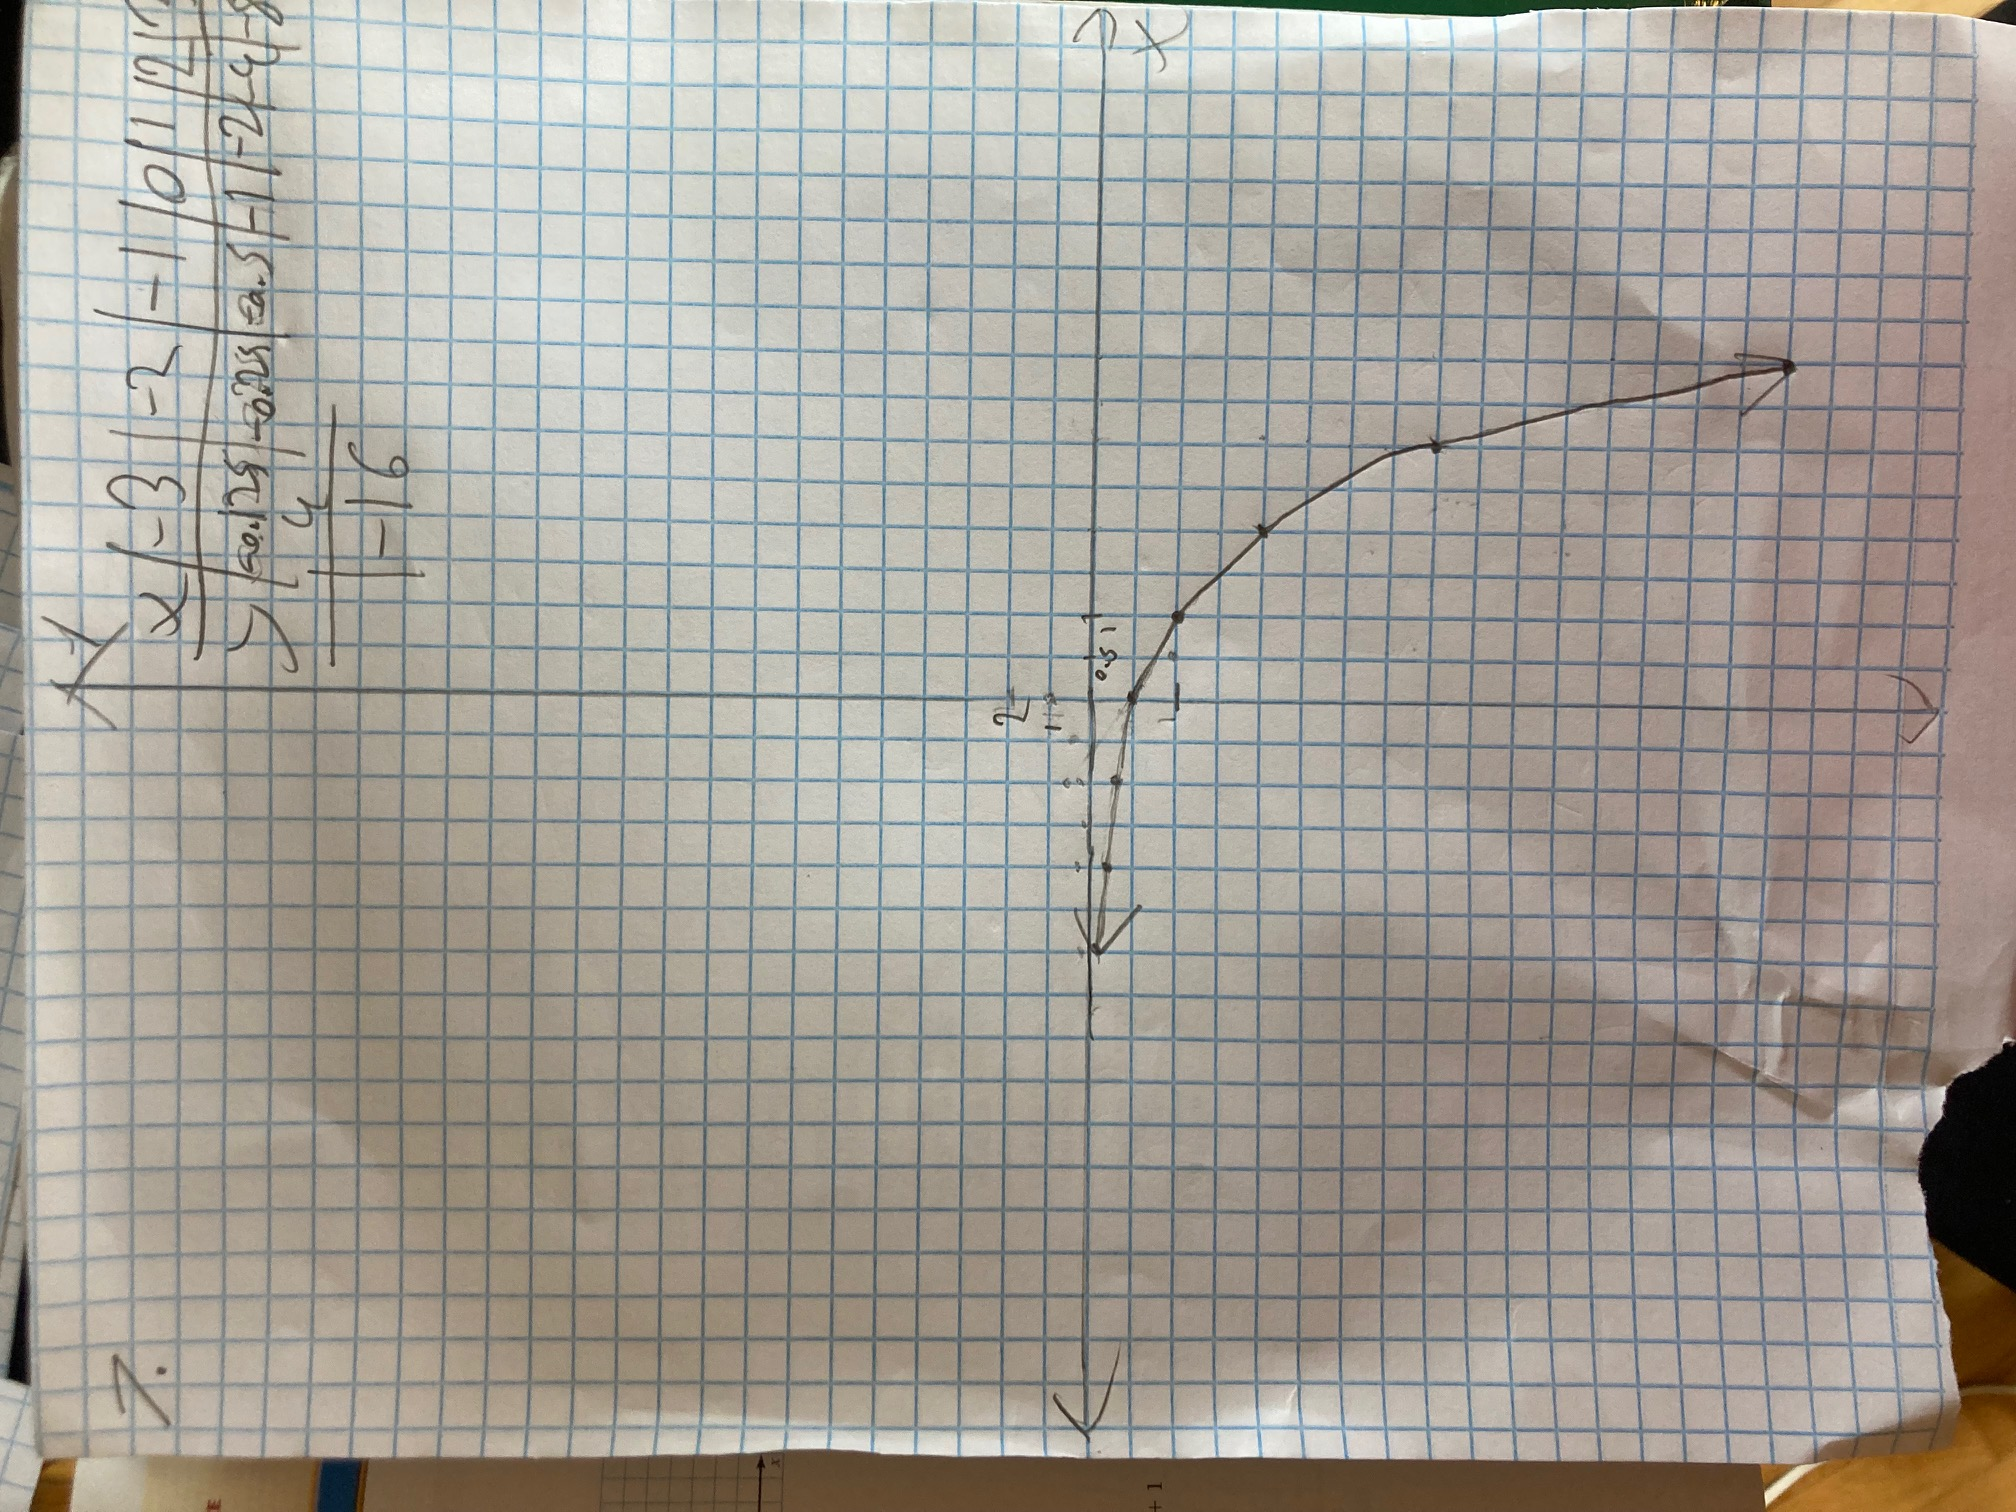
\includegraphics[width = 4in, height = 4in, angle=-90]{7}
\newline The domain of this function is all real numbers, while the range of the function is $-\infty <x<0$, as the asymptote of this function is 
$y=0$.

\section*{18}
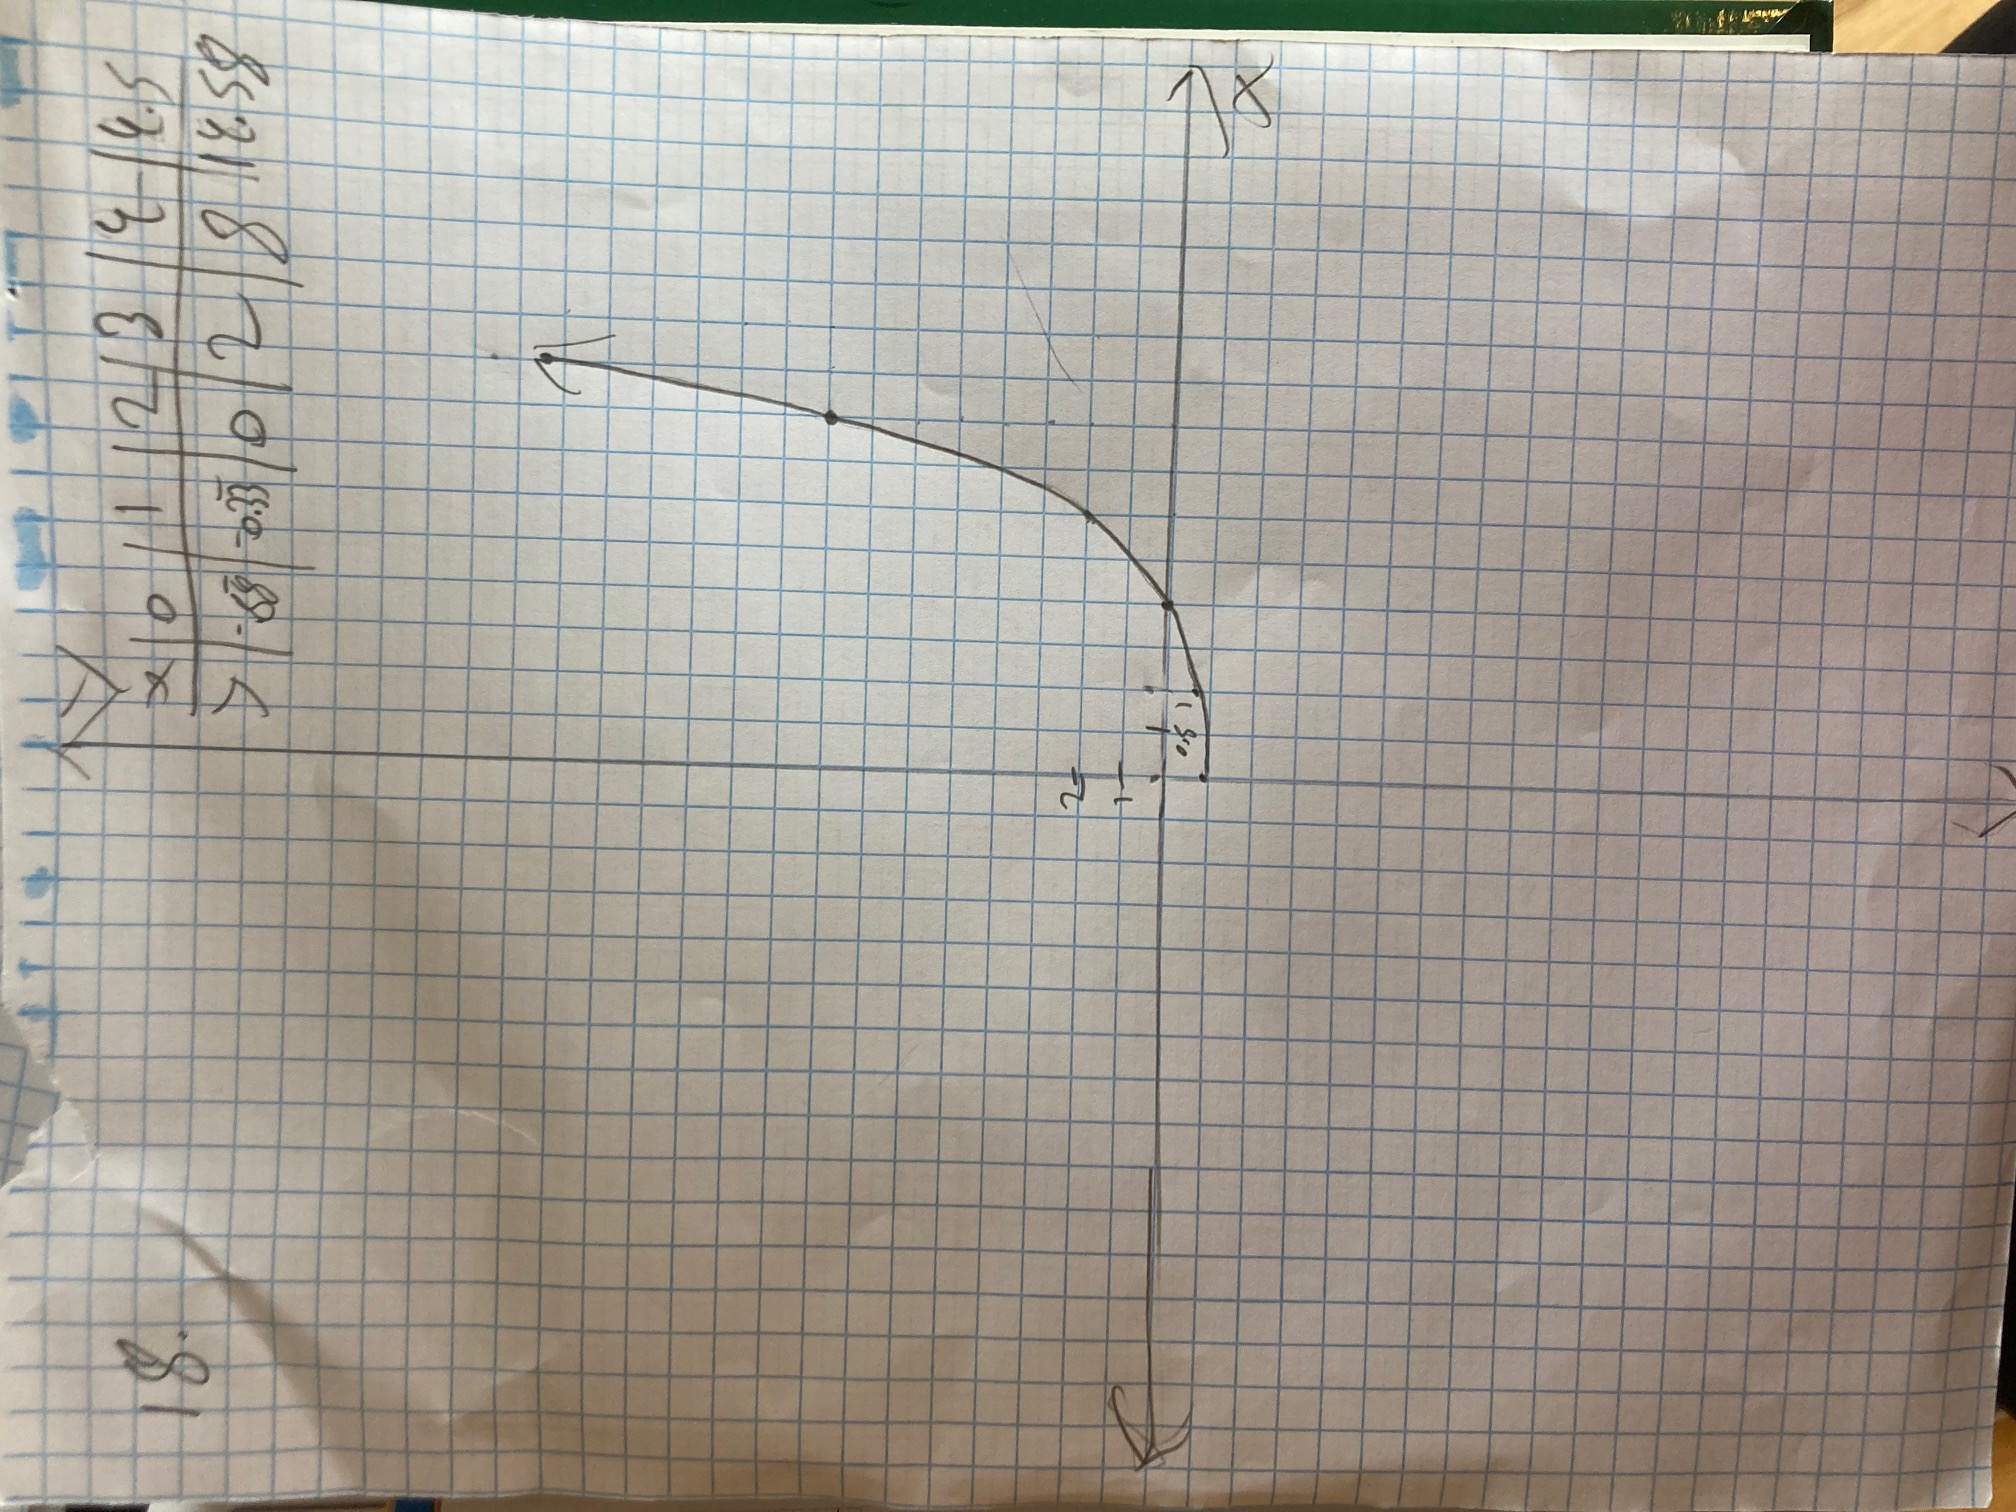
\includegraphics[width = 4in, height = 4in, angle=-90]{18}
\newline The domain of this function is all real numbers, while the range of the function is $-1<x<+\infty$, as the asymptote of this function is 
$y=-1$.

\section*{24}
B

\section*{25}
D

\section*{30}
\[ A=450(1.06)^t \]

\section*{32}
We are given an equation of the form $y=ab^{x-h}+k$, and wish to have a $y$-intercept of $5$. Thus, when $x=0$, $y=5$. Also, the asymptote of the 
graph is $y=2$. So, we let $k=2$. Thus: \[ 5=ab^{-h}+2 \] We let $a=1,h=2$, meaning:
\[ 5=b^{-2}+2 \] \[ b=\sqrt[-2]{3}=\frac{1}{\sqrt{3}}=\frac{\sqrt{3}}{3} \] meaning one such equation is:
\[ y=(\frac{\sqrt{3}}{3})^{x-2}+2 \]

\section*{34}
(a): \[ \frac{f(x+1)}{f(x)}=\frac{ab^{x+1}}{ab^x}=b \] 
(b): If the table corresponded to an exponential function of the form $ab^x$, then \[ \frac{f(1)}{f(0)}=b,b>1 \] But
\[ \frac{f(1)}{f(0)}=\frac{4}{4}=1 \] meaning this does not occur.

\section*{40}
(a): \[ p=50(1.105)^t \]
(b): The price after $5$ bids will be \[ 50(1.105)^5\approx \$ 82.37 \] According to the model, the price after 100 bids will be:
\[ 50(1.105)^{100}\approx \$ 1084420.72 \] This price does not make sense, as the model only accounts for the first 6 bids.

\section*{41} 
(a): \[ 48.28(1.06)^t \]
(b):\newline 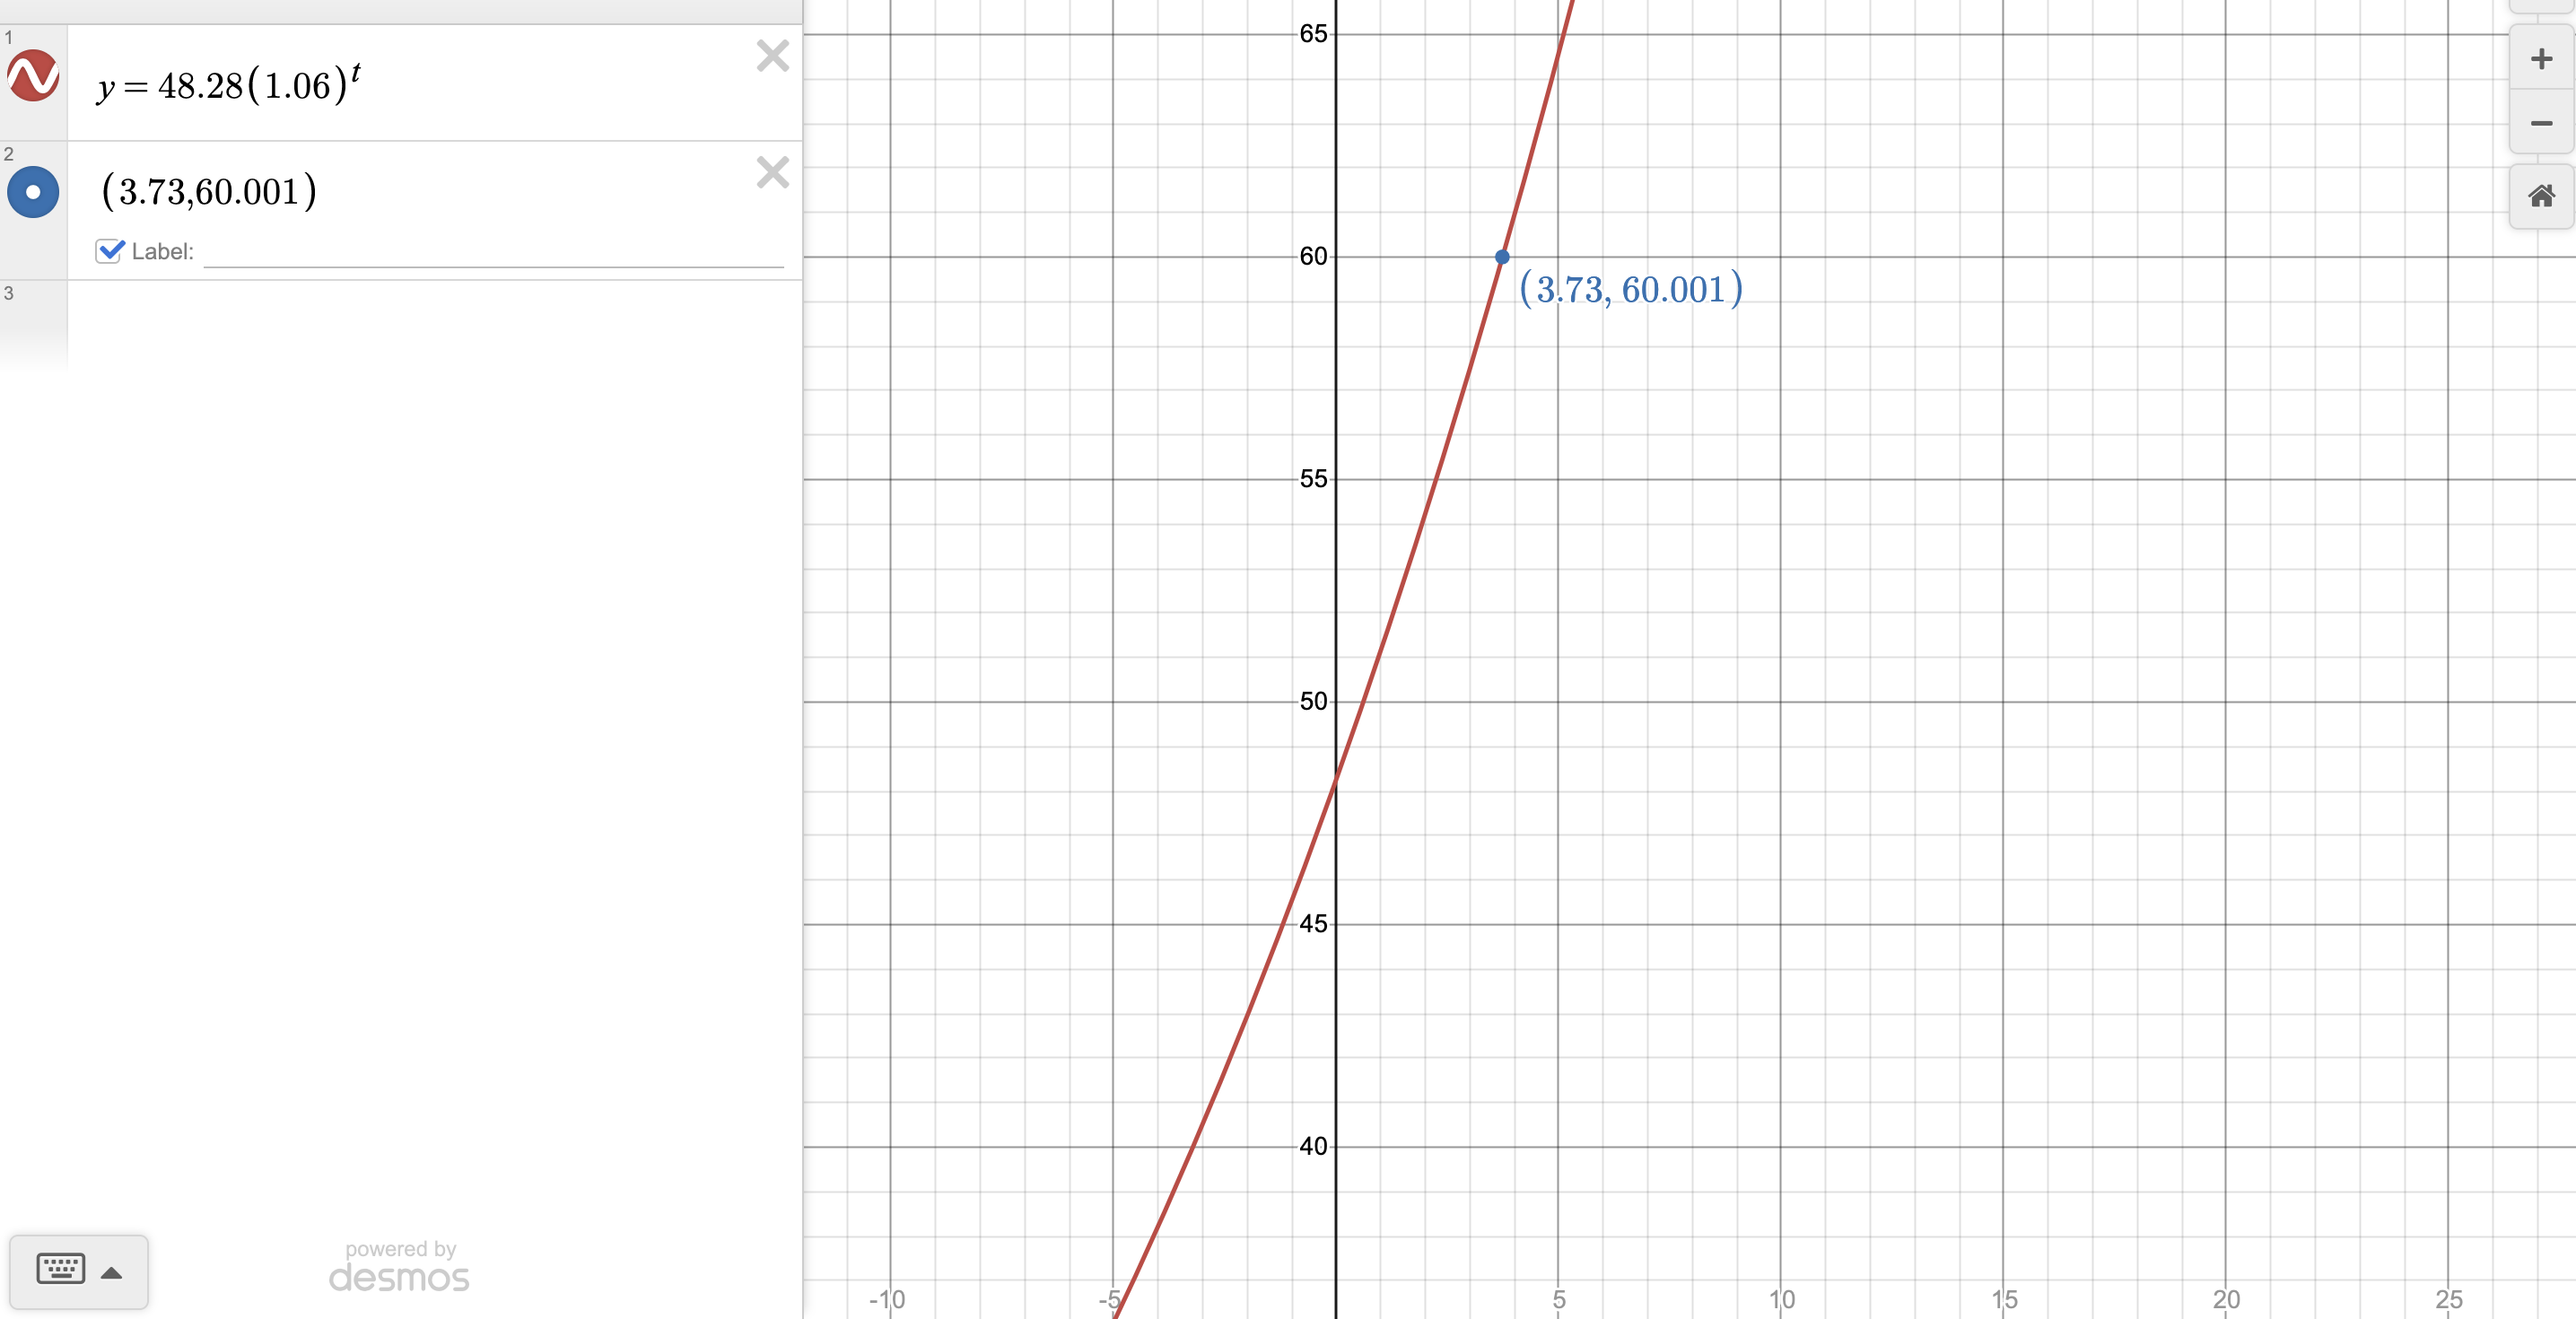
\includegraphics[width = 4in, height = 4in]{41} 
\newline From the graph, a price of about $\$ 60$ will be reached after about 3.73 years.\newline
(c): We know that the model only goes from $2000$ to 4 years after $2000$. Thus, the minimum value will be the value when $x=0$, while the maximum value 
will be the value when $x=4$.

\section*{43}
(I was not sure what "equivalent" meant here, and was unsure how to solve the problem.)\newline
The compounded interest of the first investment can be modeled by the equation: \[ A=3000(1.06)^t \]
The compounded interest of the second investment can be modeled by: \[ A=3000(1.08)^t \]
Thus, the combined total of the first two investments after $t$ years is: \[ 3000(1.06)^t+3000(1.08)^t \]
We are asked to see if this is equivalent to the third investment, which can be modeled by:
\[ A=6000(1.07)^t \]
Suppose they are equal:
\[ 6000(1.07)^t=3000(1.06^t+1.08^t) \]
\[ 2(1.07)^t=1.06^t+1.08^t \]

\section*{44}
(a): To find the growth rate, we can solve the following equation:
\[ 9000=5200(1+r)^5 \] \[ \sqrt[5]{\frac{9000}{5200}}=1+r \] \[ r\approx 0.1 \]
(b): We have now found a model for the growth rate: \[ A=5200(1.1)^t \] meaning the cost after 5 more years (after 10 years) will be about:
\[ 5200(1.1)^{10}\approx \$ 13487.46 \]

\end{document}
